\section{Vectorization}\label{sec:vector}
%Justin%
%Josh%

\subsection{Timing After Vectorization}
In order to vectorize properly vectorize our code, we looked at the output of \texttt{ipo\_out.optrpt} after compiling with flags \texttt{-qopt-report=5 -qopt-report-phase=vec}. We first were able to vectorize our call to \texttt{square} within \texttt{shortest\_paths} within \texttt{path.c} by explicitly precomputing the transpose of \texttt{l} during each call to \texttt{square}, and then replacing the assignment of \texttt{lik} directly from \texttt{l}, as
\begin{gather*}
\texttt{int lik = l[k*n+i]}
\end{gather*}
to an assignment instead from the transpose, as
\begin{gather*}
\texttt{int lik = l\_T[i*n+k]}
\end{gather*}
We also attempted to solve the issue of unaligned memory access from within \texttt{l} and \texttt{l\_T} by replacing calls to \texttt{malloc} with \texttt{\_mm\_malloc} (and, correspondingly, calls to \texttt{free} with calls to \texttt{\_mm\_free}), using a byte alignment of 32 since we're compiling with AVX2 (using the flag \texttt{-xcore-avx2}). This solved some of the issues with unaligned access, according to the vectorization report, but there are still cases with unaligned access reported.

\subsection{Timing After Vectorization}

\begin{figure}[H]
    \centering
    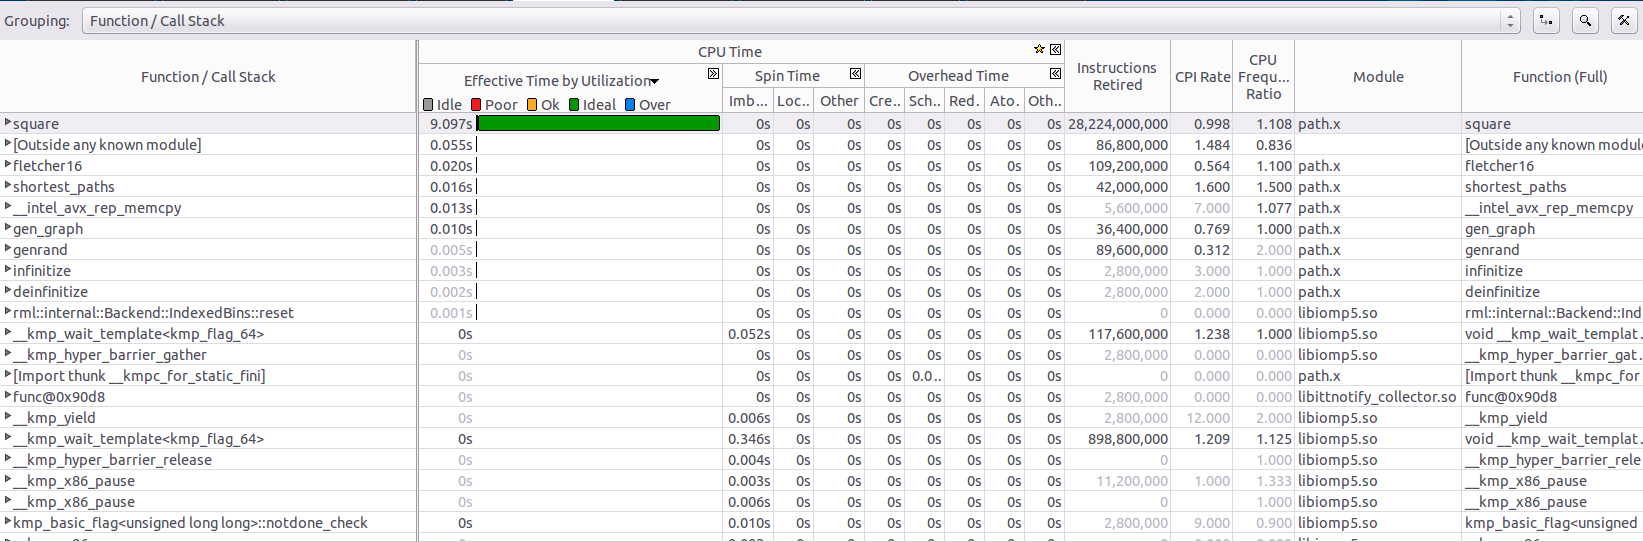
\includegraphics[width=0.8\textwidth]{figs/1_analysis.png}
    \caption{Profile Analysis After Vectorization}
    \label{vectorized_profile_result_0}
\end{figure}

As show in the picture, for the same problem size, the function \texttt{square} is more than 5
times faster than it was before, when we are running it with in Vtune, where one core is used to
trace other threads. In fact, running it with command line and time it with build in function
\texttt{omp\_get\_time()} shows the saving gives us a factor of more than 9 times faster.

\begin{figure}[H]
    \centering
    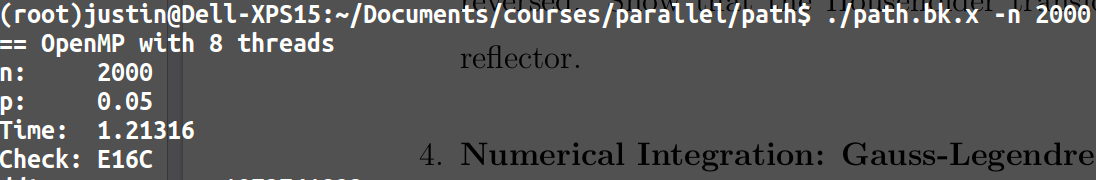
\includegraphics[width=0.8\textwidth]{figs/1_timing.png}
    \caption{Timing Result After Vectorization}
    \label{vectorized_profile_result_1}
\end{figure}

\begin{figure}[H]
    \centering
    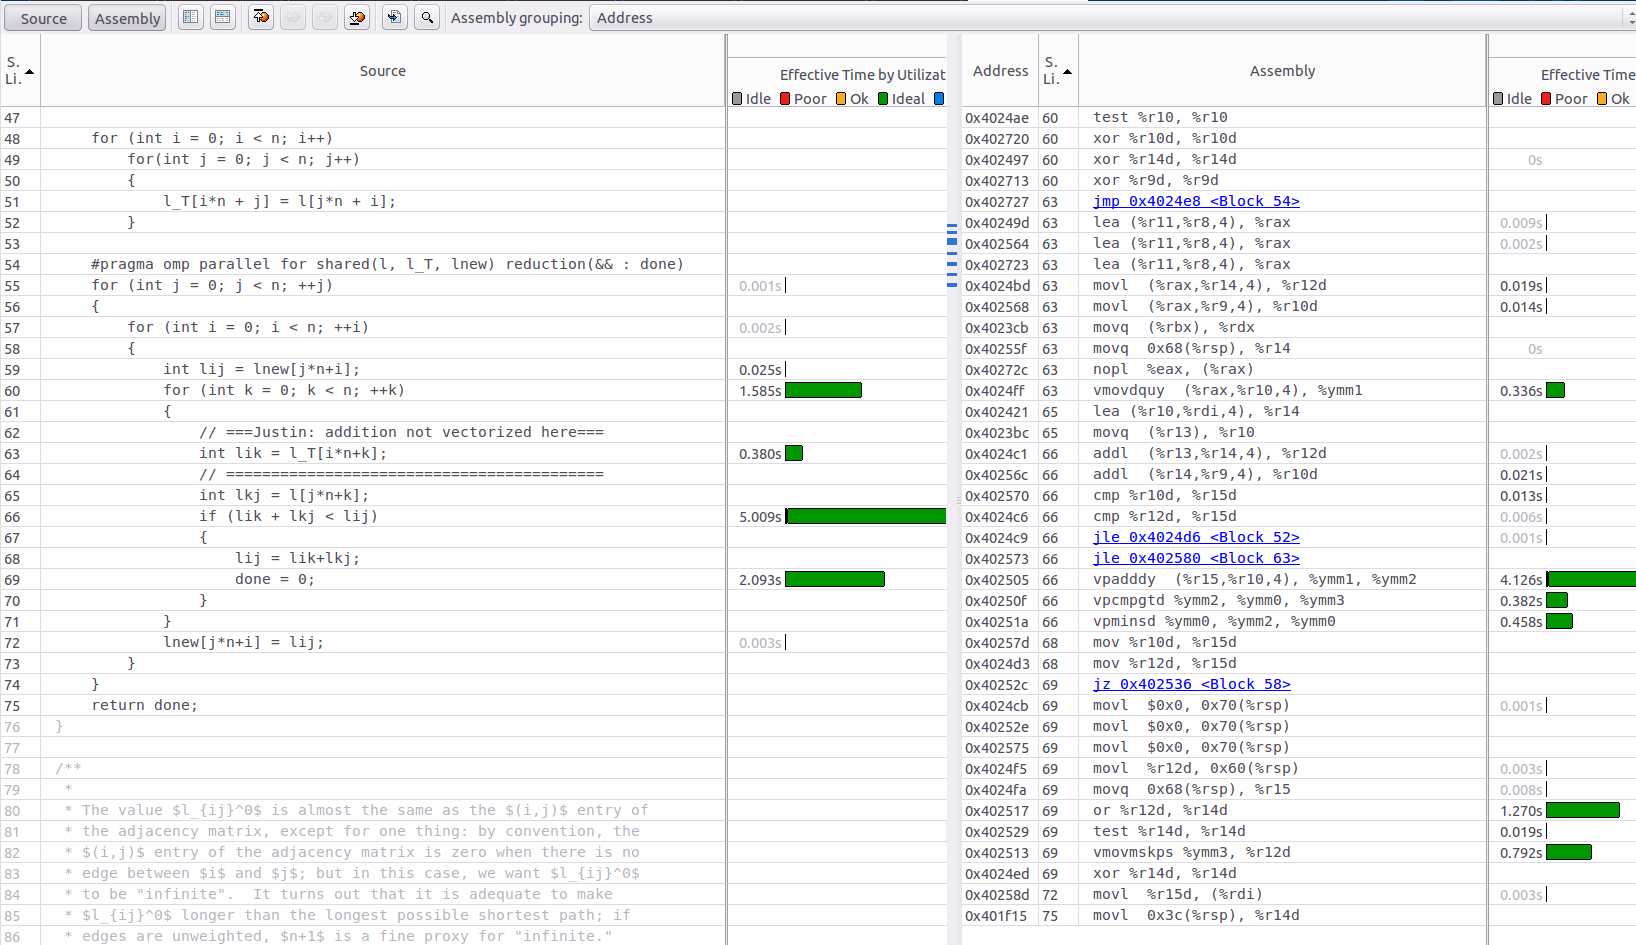
\includegraphics[width=0.8\textwidth]{figs/1_assembly.png}
    \caption{Assembly Analysis After Vectorization}
    \label{vectorized_profile_result_2}
\end{figure}

The assembly analysis is more informative as it tells how well our functions have been vectorized
as well as the timing. From the assembly analysis after vectorization, we can tell that the computations
in the inner has been vectorized. Which is where the savings come from.



\subsection{Data-Type Optimization}
As we went through tests, we found that the maximum distance between two vertices is
always below 20, even when we are calculating a 10000 by 10000 graph. Then it naturally
follows that, we don't necessarily need a 4-byte \textcolor{blue}{int} to store the
distance information. \\

To fit more data into register so that we can carry out more operation per cycle, we used
a prototype called \textcolor{blue}{ddt}, which can be any data type such as \textcolor{blue}{long},
\textcolor{blue}{short}, and \textcolor{blue}{char}. In fact, this gives us 30\% saving when we are
using \textcolor{blue}{char} to store the distance between two vertices. \\

Notice in Figure 8, we printed out a variable called \texttt{ddt\_upper\_range} which tells us the largest
distance we can have, in order to use one certain data-type. In the case with \textcolor{blue}{char}, the
largest distance is 127, which is proved to be more than enough by our tests.


\subsection{Tuned OpenMP Timing Result}

\begin{figure}[H]
    \centering
    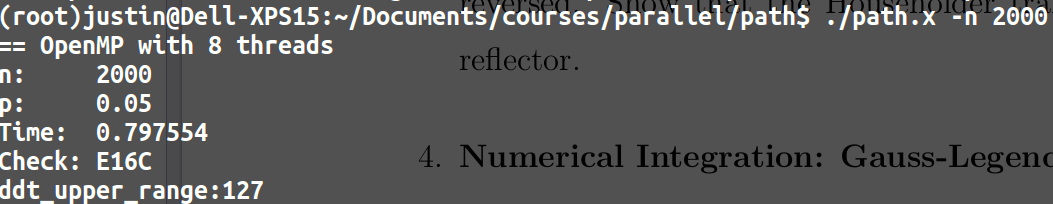
\includegraphics[width=0.8\textwidth]{figs/2_timing.png}
    \caption{Timing Result After OpenMP tuning}
    \label{ddt_profile_result_2}
\end{figure}

Timing result before introducing MPI is shown in Figure \ref{ddt_profile_result_2}.
As we can see the program is running with 8 threads using OpenMP and it takes 0.7976
seconds for 2000 vertices.

\subsection{Tuned OpenMP Profiling Result}

\begin{figure}[H]
    \centering
    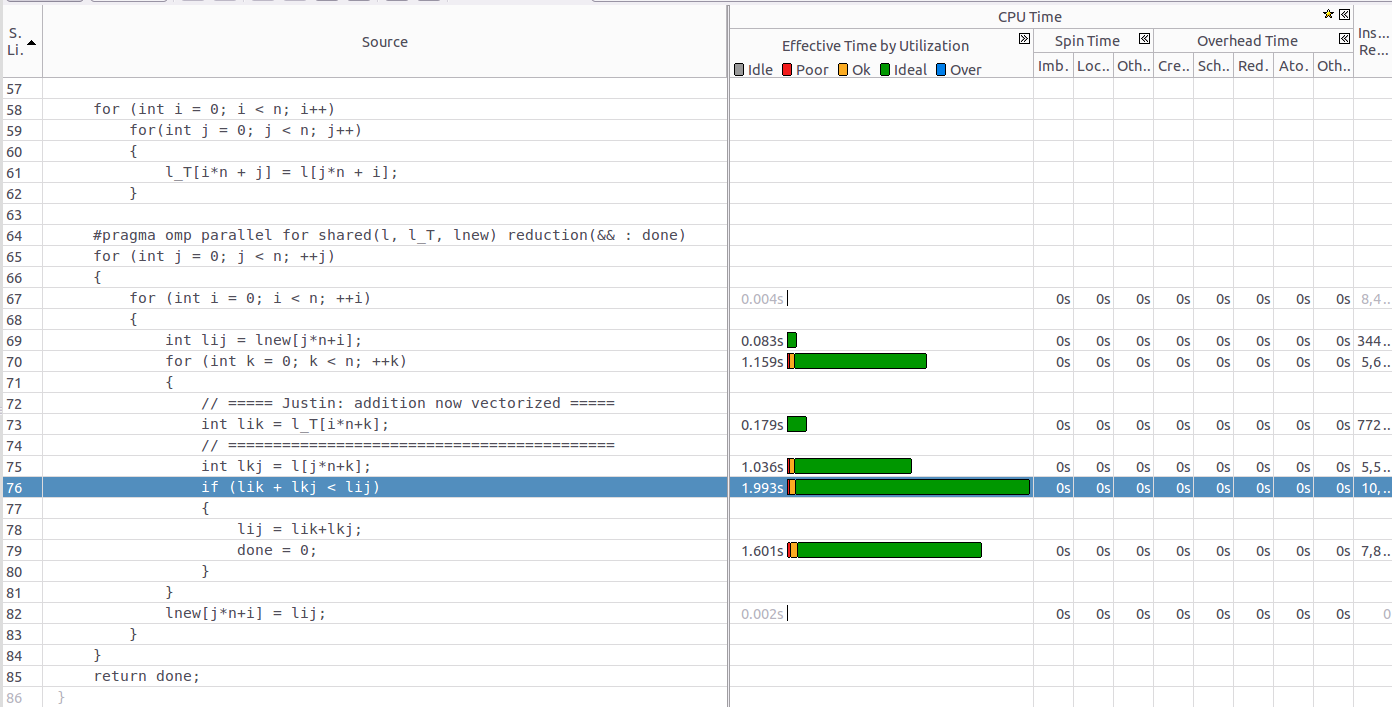
\includegraphics[width=0.8\textwidth]{figs/2_assembly.png}
    \caption{Initial Assembly Result}
    \label{ddt_profile_result_1}
\end{figure}

The assembly analysis after using data-type \textcolor{blue}{char} is down below. Comparing with Figure
\ref{vectorized_profile_result_2}, we can tell that the major saving comes from the addition between 
\texttt{lij} and \texttt{ljk}, which consist with what we would expect, since we can now fit more additions
into vector register to be calculated in one cycle.

